% Author: Martin Thoma
\subsection{Algorithmus von Kruskal}
\begin{frame}{Algorithmus von Kruskal}{Kruskal's algorithm}
	$E$: Menge der ausgewählten Kanten, $S$: Menge der erreichbaren Knoten.\vspace{10pt}\pause

	So lange, bis alle Knoten erreichbar sind:

	Wähle Kante mit geringstem Gewicht

	Wenn durch ausgewählte Kante ein Knoten erreichbar ist, der davor nicht in $S$ war, füge diese Kante zu $E$ und Knoten zu $E$ hinzu.
\end{frame}


\begin{frame}{Algorithmus von Kruskal}{Kruskal's algorithm}
	\begin{figure}
		\begin{tikzpicture}[scale=1.8, auto,swap]
			% Draw a 7,11 network
			% First we draw the vertices
			\foreach \pos/\name in {{(0,2)/a}, {(2,1)/b}, {(4,1)/c},
				                    {(0,0)/d}, {(3,0)/e}, {(2,-1)/f}, {(4,-1)/g}}
				\node[vertex] (\name) at \pos {$\name$};
			% Connect vertices with edges and draw weights
			\foreach \source/ \dest /\weight in {b/a/7, c/b/8,d/a/5,d/b/9,
				                                 e/b/7, e/c/5,e/d/15,
				                                 f/d/6,f/e/8,
				                                 g/e/9,g/f/11}
				\path[edge] (\source) -- node[weight] {$\weight$} (\dest);
			% Start animating the vertex and edge selection.
			\foreach \vertex / \fr in {d/1,a/1,e/2,c/2,f/3,b/4,g/10}
				\path<\fr-> node[selected vertex] at (\vertex) {$\vertex$};
			% For convenience we use a background layer to highlight edges
			% This way we don't have to worry about the highlighting covering
			% weight labels.
			\begin{pgfonlayer}{background}
				\pause
				\foreach \source / \dest / \fr in {a/d/1,c/e/2,d/f/3,a/b/4,b/e/6,e/g/10}
				    \path<\fr->[selected edge] (\source.center) -- (\dest.center);
				\foreach \source / \dest / \fr in {d/b/5,b/c/7,d/e/8,e/f/9,f/g/11}
				    \path<\fr->[ignored edge] (\source.center) -- (\dest.center);
			\end{pgfonlayer}
		\end{tikzpicture}
	\end{figure}
\end{frame}
%% end of source

\begin{frame}[fragile]
\frametitle{Algorithmus von Kruskal}
\begin{lstlisting}
s is disjunct set of edges
n is number of edges in original graph
while s less than n - 1
e = smallest weight edge not deleted yet
    // edge e = (u, v)
    uset = s.find(u)
    vset = s.find(v)
    if (uset != vset)
        edgesAccepted = edgesAccepted + 1
        s.unionSets(uset, vset)
    end if
end while
\end{lstlisting}
\end{frame}

\begin{frame}{Algorithmus von Kruskal}{Kruskal's algorithm}
	Erfunden von:

	1956: Joseph Kruskal

	\begin{figure}
		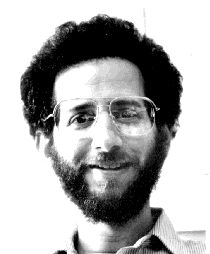
\includegraphics[scale=0.6]{Material/kruskal.jpg}
		\caption{Kruskal}
	\end{figure}
\end{frame}
